\documentclass[12pt]{article}

\usepackage{amsmath}
\usepackage{amssymb}
\usepackage{calc}
\usepackage{units}
\usepackage{graphicx}
\usepackage[pdftex]{hyperref}
\usepackage{subfig}
\usepackage[margin=1in]{geometry}
\usepackage{listings}
\usepackage[numbers,sort&compress]{natbib}
\usepackage{bm}
\usepackage{paralist}
\usepackage[draft]{fixme}
\usepackage{textcomp}
\usepackage{yorkdefs}

\newcommand{\halflife}{\ensuremath{T_{\nicefrac{1}{2}}}\xspace}

\hypersetup{
  breaklinks=true,
  pdftitle={Alternating Current RC Circuits},
  pdfauthor={Kevin R. Lynch based on a lab by D.C.Jain}, 
  pdfsubject={Phyiscs, Electricity and magnetism},
  pdfkeywords={resistance, capacitance, alternating current},
  pdflang={en-US},
}

\title{Alternating Current RC Circuits}
\author{}
%Kevin R. Lynch, based on an earlier lab by D.C.Jain
%\date{2012-03-07}
\date{}

\begin{document}

\maketitle

\section{Objectives}
\label{sec:objectives}

\begin{enumerate}
\item To understand the voltage/current phase behavior of RC circuits
  under applied alternating current voltages, and
\item To understand the current amplitude behavior of RC circuits
  under applied alternating current voltages.
\end{enumerate}

\section{Introduction}
\label{sec:introduction}

While you have studied the behavior of RC circuits under direct
current conditions, very few interesting circuits have purely direct
currents and constant applied voltages.  All productive or interesting
circuits operate under alternating current conditions - think
computers, radios (including cell phones), etc.

\begin{figure}
  \centering
  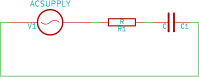
\includegraphics[width=2\textwidth/3]{figures/rc-circuit}
  \caption{The RC circuit.}
  \label{fig:rccircuit}
\end{figure}
In a previous lab\footnote{\textit{The Time Constant of an RC
    Circuit}} you studied the behavior of the RC circuit under
constant applied (or DC) voltages.  Here, you will study the behavior
of the same circuit under sinusoidally alternating applied (or AC)
voltages (see Figure~\ref{fig:rccircuit}).

\section{Theory}
\label{sec:theory}

\begin{figure}
  \centering
  \includegraphics[width=2\textwidth/3]{figures/phase}
  \caption{A schematic of the phase difference between the applied
    voltage $V(t)$ and the derived current $I(t)$.}
  \label{fig:phase}
\end{figure}
Let's begin analyzing this circuit the same way you analyzed the DC RC
circuit, via Kirchoff's Rules.  As before, you'll find
\begin{gather*}
  V_s(t) - V_R(t) - V_C(t) = 0\ .
\end{gather*}
Again, just as in the DC case,
\begin{align*}
  V_C(t) &= \frac{q(t)}{C} & V_R(t) &= I(t) R & I(t) =
  \deriv{q(t)}{t}\ ,
\end{align*}
leading to the differential equation
\begin{gather*}
  \deriv{q(t)}{t} + \frac{q(t)}{RC} = \frac{V_s(t)}{R}\ ,
\end{gather*}
which has the general solution
\begin{gather*}
  q(t) = e^{-t/RC} \left[ 
    q(t_0) e^{t_0/RC} + \int_{t_0}^t e^{t/RC} \frac{V_s(t)}{R} \dd t
\right]\ .
\end{gather*}
If $V_s(t)$ is allowed to be any old arbitrary function, you're stuck.
But getting stuck takes all the fun out of your work, so of course,
you can't allow it to be an arbitrary function: focus on sinusoids.
This is a class of broadly useful functions - they're what come out of
the wall, they're present in electromagnetic radiation, and they are
highly amenable to mathematical manipulation and analysis.  Let's take
\begin{gather*}
  V_s(t) = V_s \cos \omega t\ .
\end{gather*}
In Appendix~\ref{sec:solutions} we'll derive the full solution; here,
you will require only the \textit{steady state response}, which gives
the time dependent charge as
\begin{gather*}
  q(t) = V_s C \frac{1}{\sqrt{1+(RC\omega)^2}} \sin( \omega t + \phi)\ ,
\end{gather*}
where $\tan \phi = 1/RC\omega$.  You know $\phi$ as a \textit{phase
  constant}.  When you calculate the current flow, $I(t)$, in this
circuit, you will find a remarkable thing:
\begin{gather*}
  I(t) = \frac{V_s}{R} \frac{RC\omega}{\sqrt{1+(RC\omega)^2}} \cos(
  \omega t + \phi)\ .
\end{gather*}
Because of the presence of the capcitor, the applied voltage $V_s(t)$
gives rise to a current which not only has a frequency dependent
amplitude, but more importantly has a different phase; see
Figure~\ref{fig:phase}.  Because $phi$ is positive, the current rises
slightly before the voltage, and we say the current \textit{leads} the
voltage, or that the voltage \textit{follows} the current.  

In our teaching labs, we don't have the tools to measure the current
profile and compare it directly to the applied voltage - remember, we
only have ammeters, voltmeters, and oscilloscopes (which behave for
most purposes like voltmeters).  To use the oscilloscope to measure
this phase difference, you must find a voltage that follows exactly in
phase with the current \ldots and you have one of those: the voltage
across the resistor.  Measuring $V_R(t)$ and comparing with $V_s(t)$
allows us to measure $\phi$.
\begin{gather*}
  V_s(t) = V_s \cos \omega t\\
  V_R(t) = V_s \frac{RC\omega}{\sqrt{1+(RC\omega)^2}} \cos( \omega t
  + \phi) = I(t) R\\
  V_C(t) = V_s \frac{1}{\sqrt{1+(RC\omega)^2}} \sin( \omega t + \phi)\ ,
\end{gather*}

\begin{figure}
  \centering
  \subfloat[][Phases]{
    \includegraphics[width=\textwidth/2-0.1in]{figures/frequency-phase}
  }
  \subfloat[][Voltage Amplitudes]{
    \includegraphics[width=\textwidth/2-0.1in]{figures/frequency-amplitudes}
  }
  \caption{The phase angle as a function of angular frequency, while
    the function amplitudes are displayed on the right.  In both
    cases, the frequency is normalized in units of $1/RC$.  The phase
    is normalized to $\pi/2$, while the amplitudes are normalized to
    $V_s$.}
  \label{fig:frequency}
\end{figure}
There is another point of interest: the behavior of the system as a
function of frequency.  In the limit that the frequency goes to zero
(that is a DC voltage), the steady state behavior of this system
should look just like the DC system you studied previously: $V_R(t)$
should go to zero, $V_s(t)$ should equal the applied voltage.  You
should check these assertions; you'll find they are true.  In the
other extreme, where the frequency gets large, you probably have no
\textit{a priori} expectations.  Plotting the behavior as a function
of frequency (see Figure~\ref{fig:frequency}), you should find that
the amplitude of $V_C(t)$ vanishes, while the amplitude of $V_R(t)$
goes to $V_s$, while the phase difference between the applied voltage
and resulting current also vanishes.  You can prove this by taking the
limits of the voltage expressions when $\omega \to \infty$.  In other
words, the circuit acts like the capacitor isn't even there!
Capacitors become transparent to currents at high frequency, and
opaque to currents at very low frequencies.

There is another way to view the complexities of voltages and currents
in AC RC circuits.  Note that the quantity $RC\omega$ is
dimensionless; in other words, $1/C\omega$ has the units of
resistance.  It \textit{isn't} a resistance (it's not a constant, for
starters), but it has the same units, and some of the same properties.
Let's define the quantity
\begin{gather*}
  X_C = \frac{1}{\omega C} = \frac{1}{2\pi f C}\ ,
\end{gather*}
which is called the \textit{capacitive reactance} of the circuit.
Next, define the \textit{impedance} $Z$
\begin{gather*}
  Z^2 = R^2 + X_C^2\ .
\end{gather*}
As it turns out, if you look only at the amplitudes of the current and
applied voltages, they are related by
\begin{gather*}
  V_s = Z I\ ,
\end{gather*}
a sort of generalized version of Ohm's Law.  Note further that
\begin{gather*}
  \tan \phi = \frac{1}{RC\omega} = \frac{X_C}{R}\ .
\end{gather*}
With these definitions, you can rewrite the voltage equations for the
resistor and capacitor as
\begin{gather*}
  V_R(t) = V_s \frac{R}{Z} \cos( \omega t + \phi) = I(t) R\\
  V_C(t) = V_s \frac{X_C}{Z} \sin( \omega t + \phi)\ .
\end{gather*}
By combining these with the definition of impedance above, you also
find
\begin{gather*}
  V_s^2 = V_R^2 + V_C^2\ .
\end{gather*}

Finally, notice that $Z$ and $\phi$ can be looked on as the magnitude
and direction respectively of a \textit{vector} that gives the
relative behavior of $V_R(t)$ and $V_C(t)$ compared to $V_s(t)$.
These vectors are called \textit{phasors}, and phasor analysis
provides a useful basis for analyzing complex AC circuits.  We will
have more to say about phasors in later labs.

\section{Procedures}
\label{sec:procedures}

\begin{figure}
  \centering
 \includegraphics[width=2\textwidth/3]{figures/curvedefs} 
  \caption{Definition of the points on the oscilloscope curve called
    out in Step~\ref{item:phase}.} 
  \label{fig:curvedefs}
\end{figure}
You should receive two multimeters (one of which should be a
BK-5460), an oscilloscope, a function generator, a
decade resistance box, and a decade capacitor box.

\begin{enumerate}
\item First, let's select component values for testing.  Choose a
  value for the capacitance between $\unit[0.06]{\mu F}$ and
  $\unit[0.1]{\mu F}$.  Select a frequency between \unit[300]{Hz} and
  \unit[600]{Hz}.  Calculate $X_C$ and choose a value for $R \approx
  1.2 X_C$.  Measure and record the values of $R$ and $C$
\item Configure the circuit for testing shown in
  Figure~\ref{fig:rccircuit}.  Insert the Simpson multimeter to record
  the AC current; except in the last two steps of the procedure, make
  sure the current remains constant throughout the experiment.
\item Using the other meter, record the frequency $f$, and the RMS AC
  voltages across the signal generator $V_s$, the resistor $V_R$, and
  the capacitor $V_C$.
\item \label{item:phase} Let's measure the phase shift between the
  current and applied voltage.  Connect the oscilloscope so as to
  measure the voltage across the resistor and signal generator; make
  sure the negtive inputs share a common reference point.  Make sure
  the two signal baselines are centered with respect to the horizontal
  and vertical axes of the oscilloscope, and adjust the voltage and
  time scales so that slightly more than one cycle of both waveforms
  is visible.  You should have a display that looks roughly like
  Figure~\ref{fig:curvedefs}.  We're going to record the differences
  between the zero crossings, and calculate the phase from these
  differences.  Record (at least!) $A_1A_3$, $A_1B_1$, and
  $B_1A_2$.\footnote{$A_2B_2$ and $B_2A_3$ are redundant with
    $A_1B_1$, and $B_1A_2$, and $A_1A_2$ should equal $A_2A_3$ if you
    have properly centered the sinusoid vertically.}  Increase the
  frequency by 50\%, and determine the phase shift again.  Double the
  initial frequency, and repeat.
\item \label{item:current}
  Next, map out the amplitude of the current response.  Without
  changing $R$ and $C$, vary the frequency over, say, ten points, and
  record the frequency, RMS voltage $V_s$ and RMS current $I$ at those
  points.  Record you observations of the amplitudes of $V_s$ and
  $V_R$ on the oscilloscope.
\end{enumerate}

\appendix

\section{Derivation of Solutions}
\label{sec:solutions}

The differential equation for the AC RC circuit is given in
Section~\ref{sec:theory}.  It has the general solution
\begin{gather*}
  q(t) = e^{-t/RC} \left[ 
    q(t_0) e^{t_0/RC} + \int_{t_0}^t e^{t/RC} \frac{V_s(t)}{R} \dd t
\right]\ .
\end{gather*}
If $V_s(t)$ is allowed to be any old arbitrary function, we're stuck.
But getting stuck takes all the fun out of your work, so of course, we
won't allow it to be an arbitrary function: we'll focus on sinusoids.
This is a class of broadly useful functions - they're what come out of
the wall, they're present in electromagnetic radiation, and they are
highly amenable to mathematical manipulation and analysis.  Let's take 
\begin{gather*}
  V_s(t) = V_s \cos \omega t\ .
\end{gather*}
From your PHYS-151 course, you should remember that $V_s$ is the
\textit{amplitude} of the oscillation, while $\omega = 2 \pi f$ is the
\textit{angular frequency}.  With this applied voltage, we
\textit{can} perform the integration, which I leave as an exercise to
the reader.\footnote{Hint:
  \begin{gather*}
    \cos \omega t = \frac{e^{i\omega t} + e^{-i\omega t}}{2}\ .
  \end{gather*}
}

Upon integrating and collecting terms, you will find a very
complicated looking expression:
\begin{multline*}
  q(t) = q(t_0) e^{-(t-t_0)/RC} 
  - e^{-(t-t_0)/RC} \frac{V_s}{R} \frac{1}{(1/RC)^2 + \omega^2} 
  \left( \frac{1}{RC} \cos \omega t_0 + \omega \sin \omega t_0 \right) \\
  + \frac{V_s}{R} \frac{1}{(1/RC)^2 + \omega^2} 
  \left( \frac{1}{RC} \cos \omega t + \omega \sin \omega t \right)\ .
\end{multline*}
Notice that the first line contains only a decaying exponential
dependence on time; wait long enough, and those terms all die off.
This is called the \textit{transient response} of the circuit, which
comes from the initial charge on the capacitor and the initial action
of turning on the function generator at time $t_0$.  The second line
has no exponential dependence, and is called the \textit{steady state}
response of the circuit.  That's the part we are really interested in,
and it looks fairly awful in this form.  Let's clean it up some.

Consider the following expression
\begin{gather*}
  \alpha \cos \omega t + \omega \sin \omega t\ .
\end{gather*}
Both terms have the same frequency, so we should be able to rewrite
this as a single sinusoid, with a phase shift
\begin{gather*}
  A \sin (\omega t + \phi)\ .
\end{gather*}
Applying the trigonometric angle addition identities, we find
\begin{gather*}
  A \sin (\omega t + \phi) = A \sin\phi \cos\omega t + A \cos\phi
  \sin\omega t\ .
\end{gather*}
Equating terms in this expression with the first expression in the
paragraph, you find
\begin{align*}
  \alpha &= A \sin\phi & \omega &= A \cos\phi\ .
\end{align*}
Solving for $A$ and $\phi$, you should obtain
\begin{align*}
  A &= \sqrt{\alpha^2 + \omega^2}  & \tan\phi &=
  \frac{\alpha}{\omega}\ .
\end{align*}
Substituting back into the steady state response in the previous
paragraph, where $\alpha = 1/RC$, we find
\begin{gather*}
  q(t)_\mathrm{ss} = V_s C \frac{1}{\sqrt{1+(RC\omega)^2}}
  \sin(\omega t + \phi)\ .
\end{gather*}

\newpage

\section*{Pre-Lab Exercises}

Answer these questions as instructed on Blackboard; make sure to
submit them before your lab session!

\begin{enumerate}
\item Calculate the reactance of a $\unit[0.01]{\mu F}$ capacitor at a
  frequency of \unit[250]{Hz}.
% 64 kOhm
\item If an RC circuit has a $\unit[50]{\Omega}$ resistor in series
  with a $\unit[1]{\mu F}$ capacitor, what will its impedance be at
  \unit[500]{Hz}?
% 320 Ohm
\item An RC circuit has a $\unit[5]{k\Omega}$ resistor and a
  $\unit[1]{\mu F}$ capacitor.  At what frequency will the current
  lead the voltage by $\pi/4$?
% 32Hz
\item An RC circuit has a $\unit[5]{k\Omega}$ resistor and a
  $\unit[1]{\mu F}$ capacitor.  This circuit is driven by a
  \unit[100]{Hz} sine wave with \unit[1]{V} amplitude.  What is the
  amplitude of the current in the circuit?
% 0.19 mA
\end{enumerate}

\newpage

\section*{Post-Lab Exercises}

\begin{enumerate}
\item Perform the integral 
  \begin{gather*}
    \int_{t_0}^t e^{\alpha t} \cos\beta t \dd t\ ,
  \end{gather*}
  where $\alpha$ and $\beta$ are constants.  What is the result?
\item From your measured resistance, capacitance, and frequency,
  determine the reactance and impedance of your circuit.  Make sure to
  estimate your uncertainties.  Determine the impedance experimentally
  via another method, taking care of the uncertaintites.% V_s/I
  Do you get the same results?
\item Estimate the uncertainties on the measured values of $V_s$,
  $V_C$, and $V_R$.  Are the three values consistent with each other?
  Explain what you mean by ``consistent''.
\item Describe qualitatively what happens to your signals when you
  vary the frequency.
\item From your measurements in Step~\ref{item:phase} of the
  procedure, determine the phase shift at each of the three measured
  frequencies, including an estimate of the uncertainty.  How do these
  compare to the theoretical predictions? 
\item Is your data from Step~\ref{item:current} consistent with the
  predictions of theory?  Specifically, do the voltage and current
  amplitudes measured by oscilloscope and by multimeter match, within
  uncertainties, and do they comport with theoretical expectations?
\item Discuss briefly whether you have met the objectives of the lab
  exercises.
\end{enumerate}

\end{document}

%%% Local Variables: 
%%% mode: latex
%%% TeX-master: t
%%% End: 
